\chapter{Resultados}



En el gráfico \ref{figure:Entrenamiento_modelos} se puede observar los resultados de la metrica micro F1 para los distintos modelos escogidos, a lo largo de su entrenamiento. Cabe resaltar que son los resultados promedio de cada modelo estos se entrenaron 10 veces cada uno cambiando su semilla. Se observa entonces que el de mejor comportamiento fue el robertuito-base-uncased con un micro f1 al final de su entrenamiento de 0.8393, siendo asi el modelo escogido.


\begin{figure}[h]
	\caption{Entrenamiento de los modelos}
	\centering
	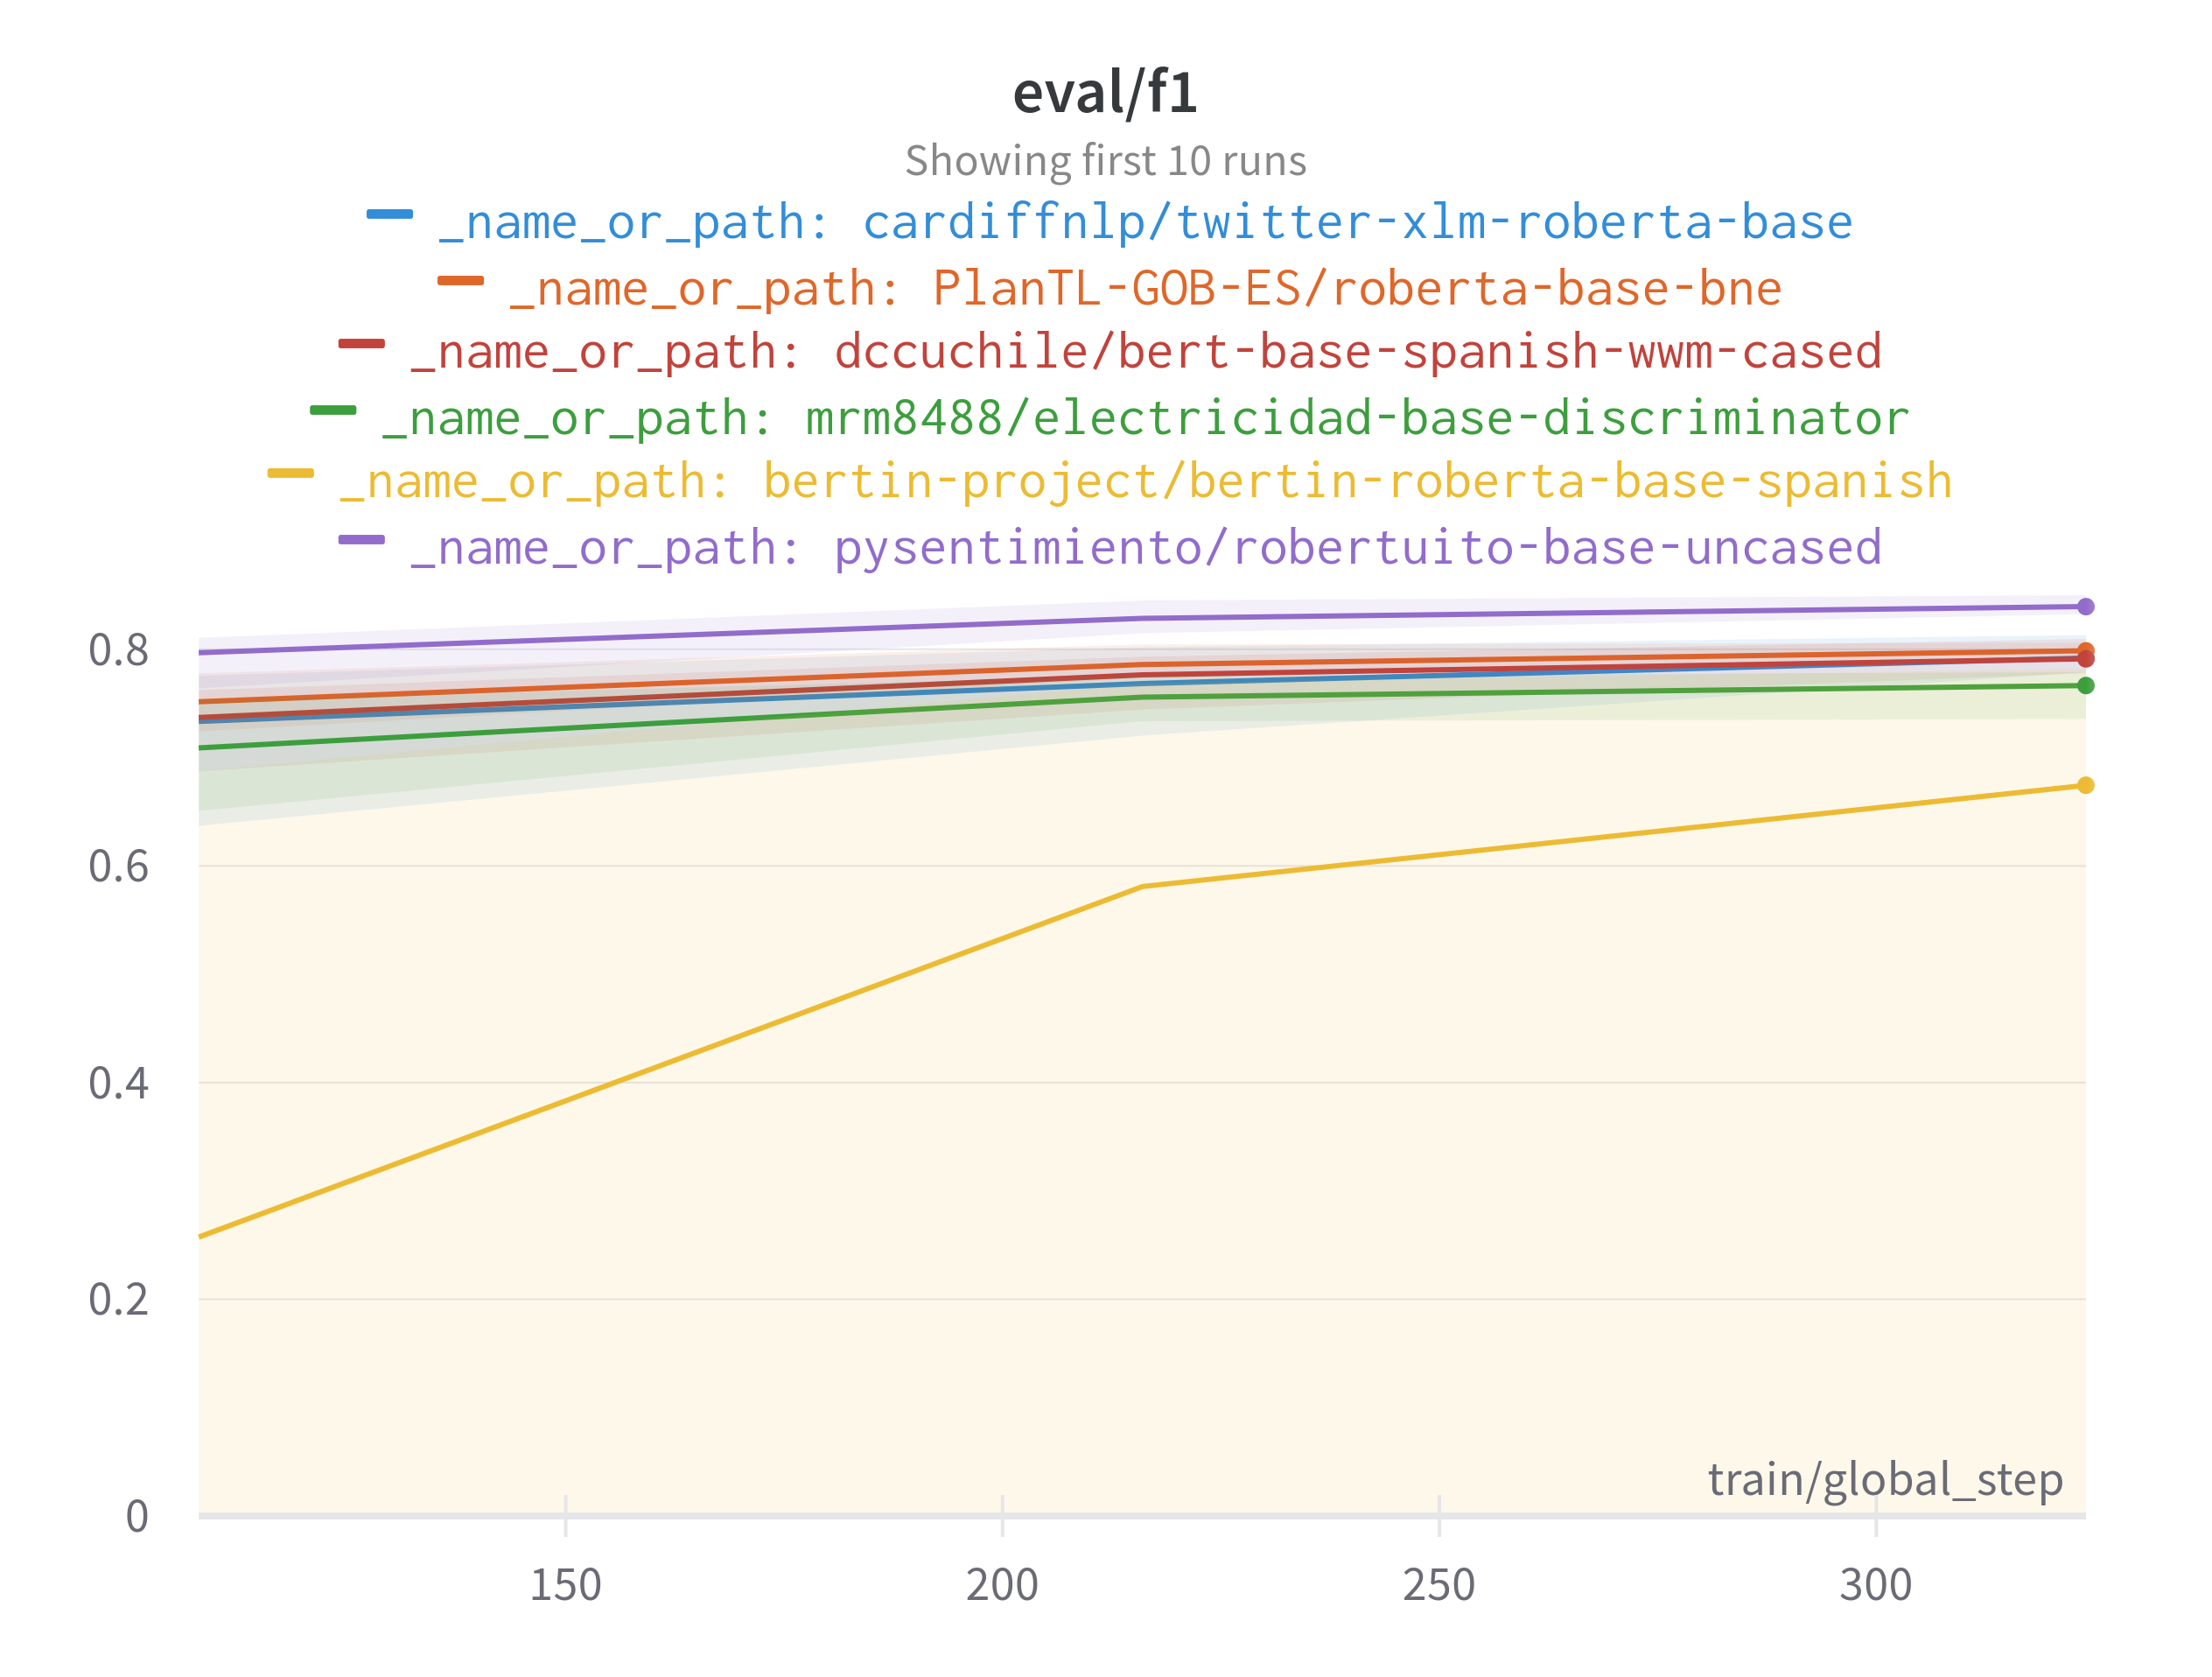
\includegraphics[scale=0.15]{../Images/Results/W&B Chart 5_18_2023, 7_25_13 PM (1).png} 
	\label{figure:Entrenamiento_modelos}
\end{figure}


\section{Distribución de emociones por sector}

Una vez desplegado el modelo y obtenido las etiquetas emocionales para todos los tweets del dataset se obtienen los resultados obtenidos en el gráfico \ref{figure:tweets_total}, en donde se aprecia el porcentaje de tweets que recibió cada una de las distintas etiquetas. Allí puede apreciarse que la emoción mas preponderante fue el asco, con mas del 50\% de los tweets. Luego fue la alegría, con alrededor del  40\%. Finalmente, el miedo y la tristeza estuvieron mucho menos presentes con menos del 3\% cada una. 

\begin{figure}[h]
	\caption{Porcentaje de tweets por emociones}
	\centering
	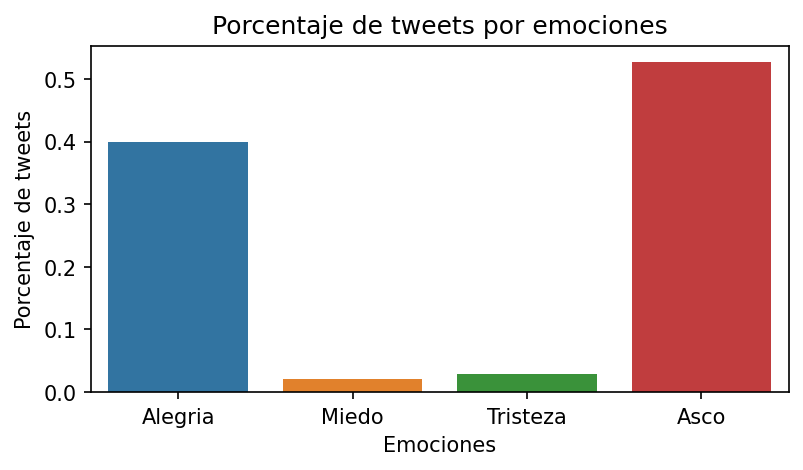
\includegraphics{../Images/Results/Cantidad_de_tweets__por_emocion.png} 
	\label{figure:tweets_total}
\end{figure}



Al analizar la presencia emocional de cada emoción en los distintos sectores políticos, se obtuvieron los resultados que se presentan en el gráfico \ref{figure:tweets_percent_miedo}. En dicho gráfico se observa que el sector neutral fue el que mostró una mayor cantidad de tweets etiquetados con miedo, representando aproximadamente el 3\% de sus tweets. En cambio, tanto la izquierda como la derecha tuvieron una presencia menor, con alrededor del 1.2\% y 0.8\% respectivamente.








\begin{figure}[h]
	\caption{Porcentaje de tweets por sector etiquetados con Miedo}
	\centering
	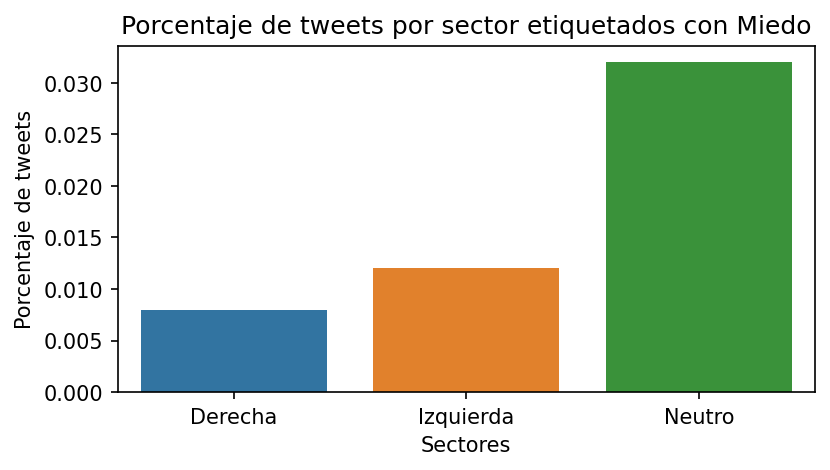
\includegraphics{../Images/Results/Porcentaje de tweets por sector etiquetados con Miedo.png} 
	\label{figure:tweets_percent_miedo}
\end{figure}

En relación a la emoción de alegría, el gráfico \ref{figure:tweets_percent_alegria} revela que la izquierda fue el sector que mostró una mayor presencia de dicha emoción en sus tweets, alcanzando el 55\%. En segundo lugar se encuentra el sector neutral, con un 33\%, seguido por la derecha con un 29\%.

\begin{figure}[h]
	\caption{Porcentaje de tweets por sector etiquetados con Alegría}
	\centering
	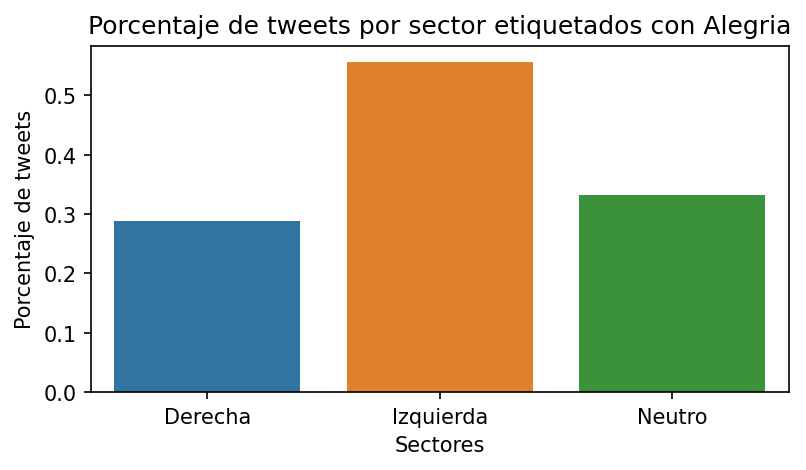
\includegraphics{../Images/Results/Porcentaje de tweets por sector etiquetados con Alegria.png} 
	\label{figure:tweets_percent_alegria}
\end{figure}

En cuanto al asco, se destaca la participación predominante de la derecha, como se observa en el gráfico \ref{figure:tweets_percent_asco}, representando un 69\% del total de sus tweets. El sector neutral se posiciona en segundo lugar con un 54\% de los tweets, dejando a la izquierda con el menor porcentaje de los tres, un 40\%.

\begin{figure}[h]
	\caption{Porcentaje de tweets por sector etiquetados con Asco}
	\centering
	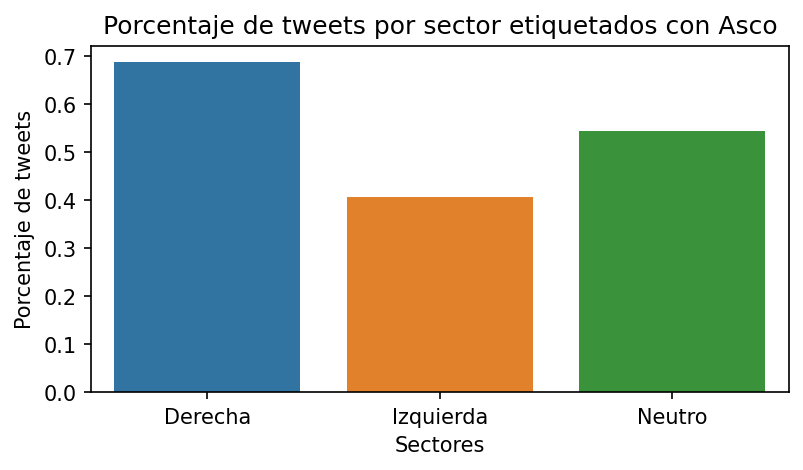
\includegraphics{../Images/Results/Porcentaje de tweets por sector etiquetados con Asco.png} 
	\label{figure:tweets_percent_asco}
\end{figure}


Finalmente, para la tristeza, el sector neutro fue en donde esta emocion tuvo mayor presencia con un 5\% de su total, lo cual fue bastante mayor que la izquierda y la derecha, con un un .08 y .04\% respectivamente.

\begin{figure}[h]
	\caption{Porcentaje de tweets por sector etiquetados con Tristeza}
	\centering
	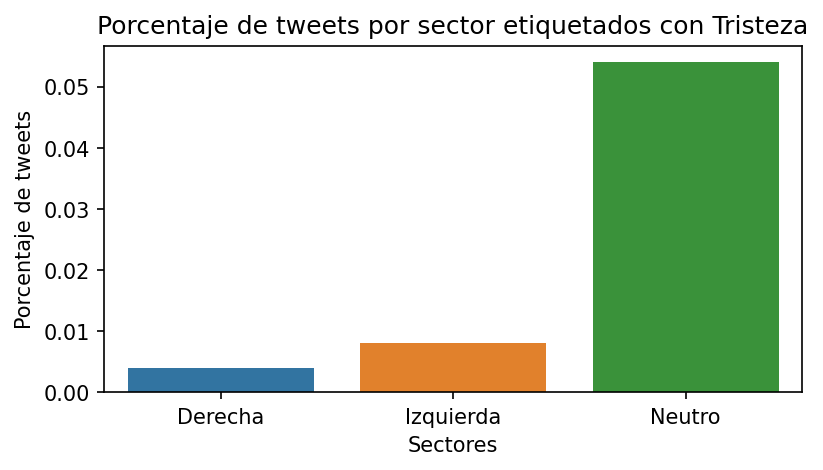
\includegraphics{../Images/Results/Porcentaje de tweets por sector etiquetados con Tristeza.png} 
	\label{figure:tweets_percent_tristeza}
\end{figure}




\section{Emociones a lo largo del tiempo}


Para determinar para cada emoción, que porcentaje de esta etiqueta tuvo un día en particular, se  dividió el numero tweets con esta emoción en dicho día sobre el total de tweets con esta etiqueta. De esta manera, se aprecia en el gráfico  \ref{figure:tweets_percent_tiempo}, que el 29 de mayo fue particularmente activo pues contó con casi 40\% de los tweets con miedo, y un 26\% de los tweets con alegría y tristeza. Este fue el día de la primera vuelta presidencial. Del mismo modo, se aprecia como los días 9 y 10 de junio tuvieron un repunte de asco y tristeza respectivamente, con un 9 y 11\%. Estos días estuvieron marcados con el evento de los llamados Petro videos. Luego hay un repunte de asco y tristeza al rededor del 16 de junio, fecha en donde se hablo del debate final al cual Rodolfo Hernandez se negó a participar, y finalmente de alegría, tristeza y miedo para el 19 de junio que fue la segunda vuelta.

\begin{figure}[h]
	\caption{Porcentaje de tweets por sector etiquetados con Tristeza}
	\centering
	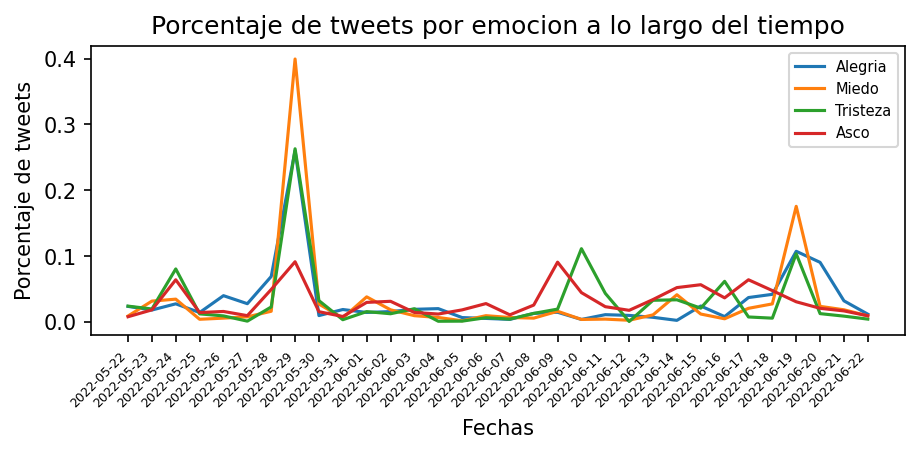
\includegraphics{../Images/Results/Porcentaje de tweets por emocion a lo largo del tiempo.png} 
	\label{figure:tweets_percent_tiempo}
\end{figure}



Para cada emoción y cada sector, se obtuvo que porcentaje de esta etiqueta tuvo este sector un día en particular, al dividir el numero de tweets que este sector tuvo con esta etiqueta en dicho día sobre el total de tweets que este sector tuvo con esta etiqueta. De esta manera, se obtiene el gráfico \ref{figure:tweets_percent_alegria_tiempo} en donde se aprecia que el 29 de mayo todos los sectores tuvieron un repunte. Luego los tres sectores van creciendo cercanos al 19 de junio, para decaer eventualmente primero la derecha, luego el sector neutro y finalmente la izquierda.




\begin{figure}[h]
	\caption{Porcentaje de tweets con Alegría por sector lo largo del tiempo}
	\centering
	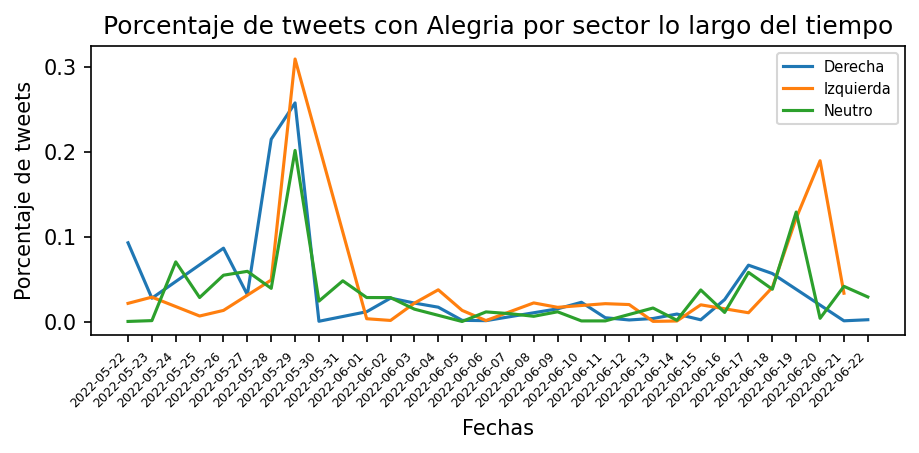
\includegraphics{../Images/Results/Porcentaje de tweets con Alegria por sector lo largo del tiempo.png} 
	\label{figure:tweets_percent_alegria_tiempo}
\end{figure}


Para el caso del miedo, se observa un gran pico de los tres sectores el 29 de mayo. Luego, para el 14 de junio, hubo un pico de miedo en la derecha como consecuencia a los rumores de estallido social, para finalmente haber un pico de miedo del sector neutro y de la izquierda cercano al 19 de junio.

\begin{figure}[h]
	\caption{Porcentaje de tweets con Miedo por sector lo largo del tiempo}
	\centering
	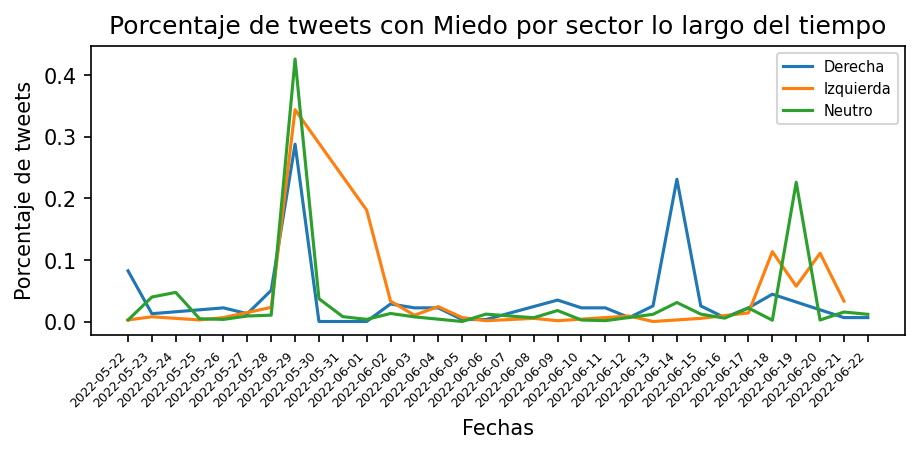
\includegraphics{../Images/Results/Porcentaje de tweets con Miedo por sector lo largo del tiempo.png} 
	\label{figure:tweets_percent_Miedo_tiempo}
\end{figure}


En cuanto a la tristeza, se aprecia que los tres sectores tuvieron un repunte el 29 de mayo, principalmente la izquierda en donde este dia se llego a casi un 40\%. Luego el 9 de junio hubo un repunte en la derecha, ligado al evento de los petro videos, y luego el 10 un repunte del sector neutro en donde se discutieron temáticas decepcionantes de las elecciones. Para el 14 de junio, la derecha tuvo devuelta un repunte de tristeza ligado, al igual que para el miedo, a la temática del estallido social. Finalmente, los tres sectores tuvieron un incremento de la tristeza para el 19 de junio.

\begin{figure}[h]
	\caption{Porcentaje de tweets con Tristeza por sector lo largo del tiempo}
	\centering
	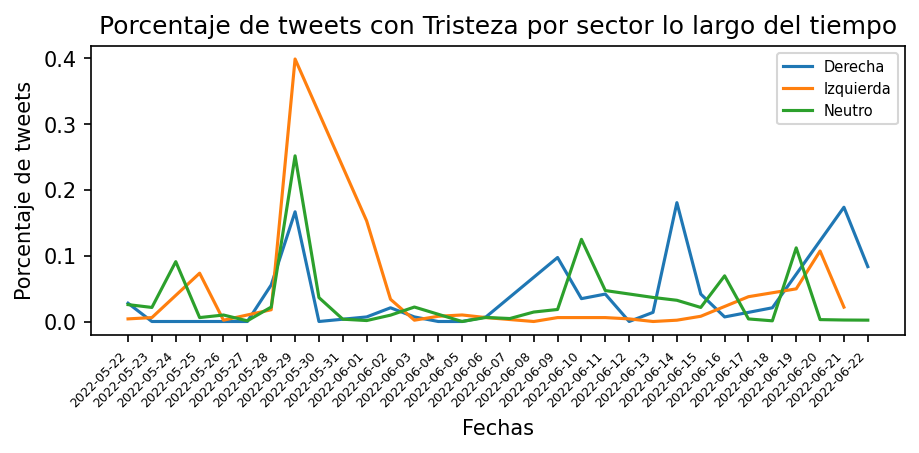
\includegraphics{../Images/Results/Porcentaje de tweets con Tristeza por sector lo largo del tiempo.png} 
	\label{figure:tweets_percent_Tristeza_tiempo}
\end{figure}

En cuanto al asco, al inicio hay un pico del sector neutro el 24 de mayo debido a las reacciones respecto a n debate. Luego, hubo un repunte de los tres sectores para el 29 de mayo. Se destaca el gran pico que tuvo la derecha, con mas del 25\%. Asi mismo, se observa que la izquierda tuvo su pico el 17 de junio con cerca del 20\%. En esta fecha fue en donde se hablo de la negativa de Rodolfo Hernandez a participar en el debate final

\begin{figure}[h]
	\caption{Porcentaje de tweets con Asco por sector lo largo del tiempo}
	\centering
	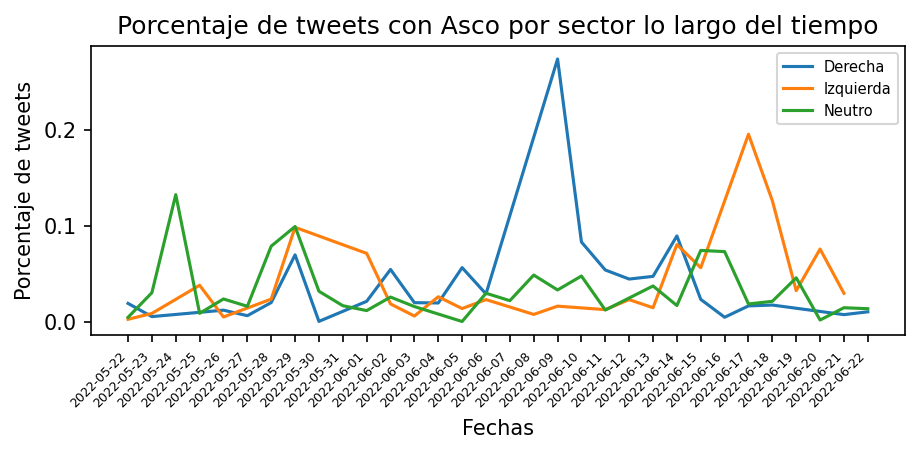
\includegraphics{../Images/Results/Porcentaje de tweets con Asco por sector lo largo del tiempo.png} 
	\label{figure:tweets_percent_Asco_tiempo}
\end{figure}














